\section{Exercise 2: Progressive Growing of GANs}

By now, you probably have realized how difficult it can be to train
GANs. They are fairly unstable, especially when trying to generated high
dimensional samples, such as high resolution images! \newline 

However, researchers never lack ideas to improve them and this 2017
paper made trainings of GANs more stable:
\href{https://arxiv.org/pdf/1710.10196.pdf}{Progressive growing of GANs
for improved quality, stability and variation}. \newline

The main idea behind this paper is the following: since training GANs on
smaller images is easier, we can progressively grow the network and the
generated images dimensions to make training easier for the network. It
is illustrated by the figure below:

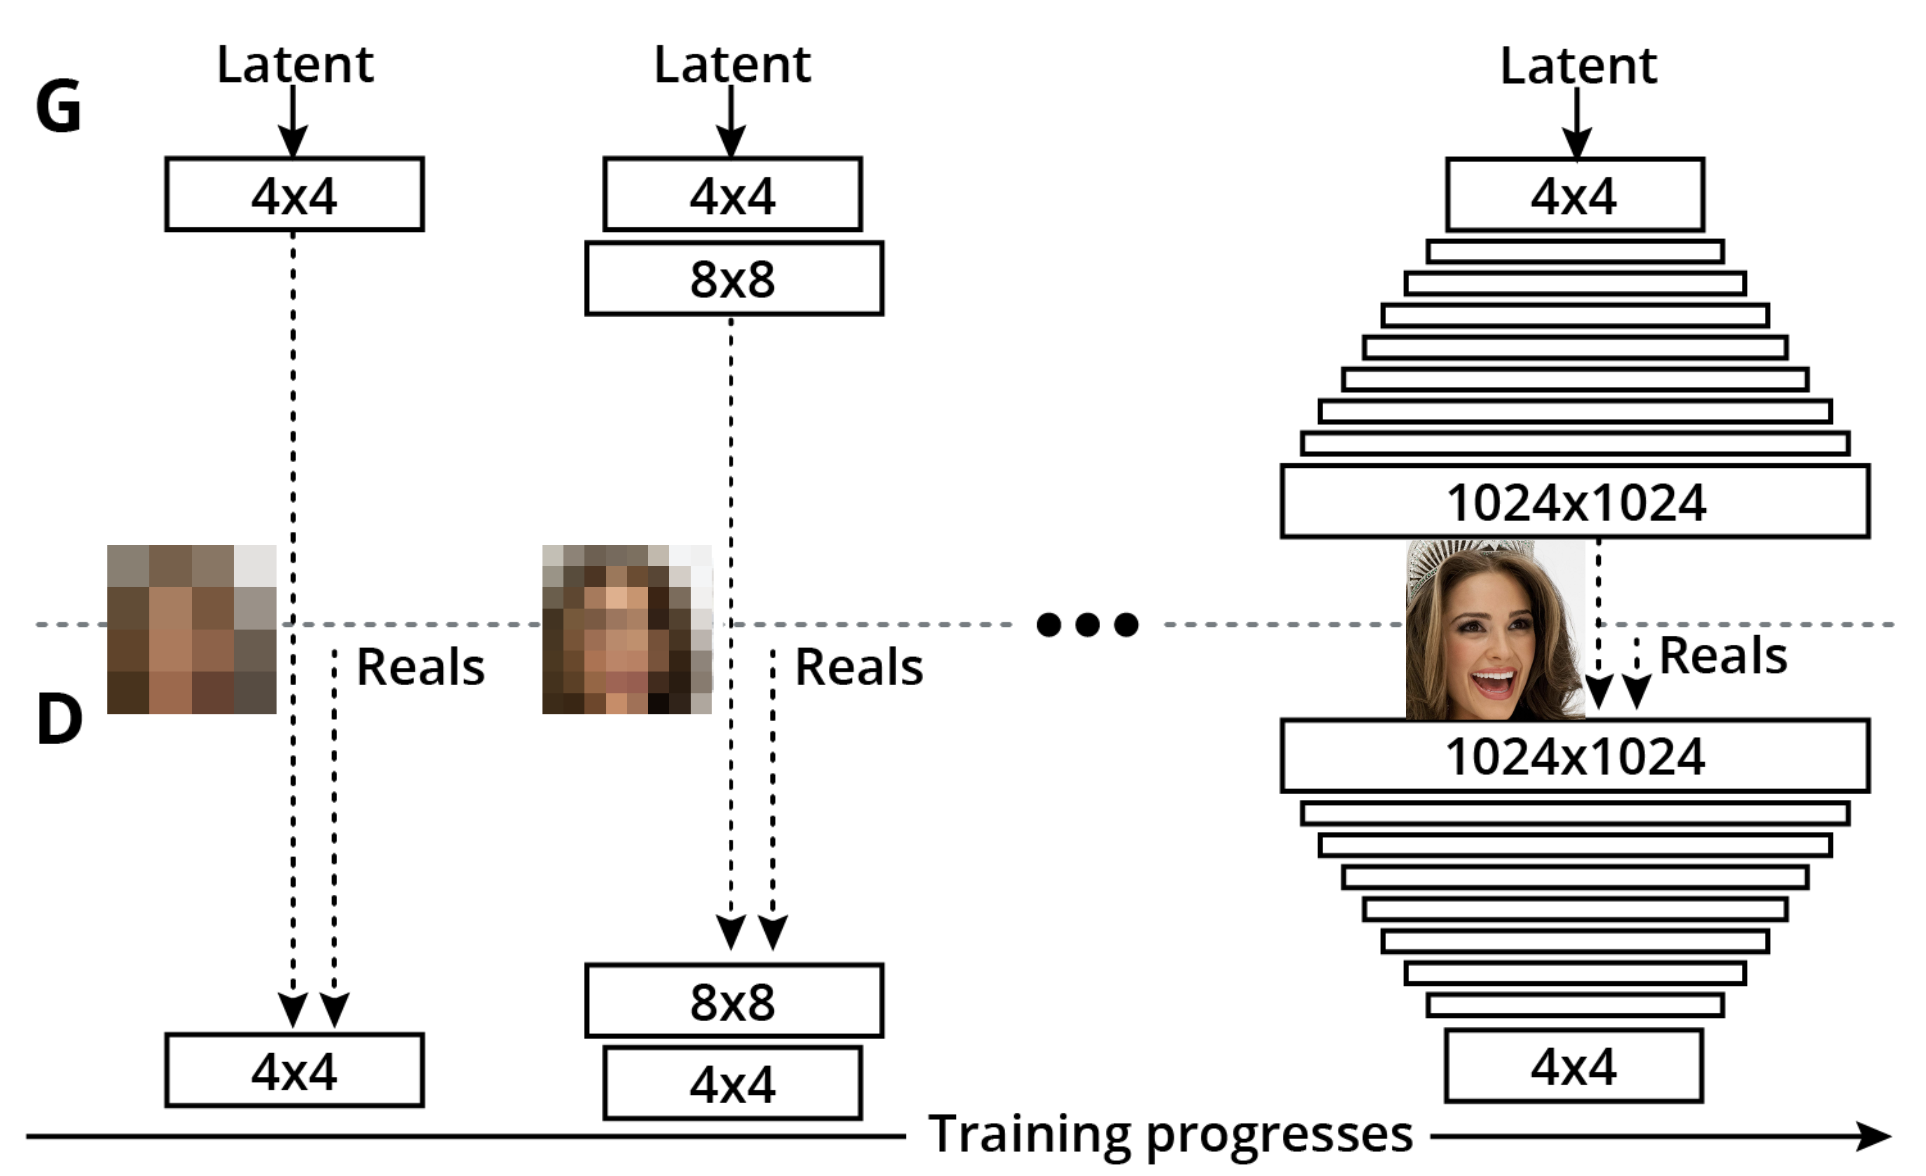
\includegraphics[width=1\linewidth]{img//genAdvNet//modernGAN/progan2.png}

\subsection{Layer fading}
Each level, or depth, is training for a certain number of epochs (eg, 10
epochs). Then a new layer is added in the discriminator and the
generator and we start training with these additional layers. However,
when a new layer is added, it is fadded in smoothly, as described by the
following figure:

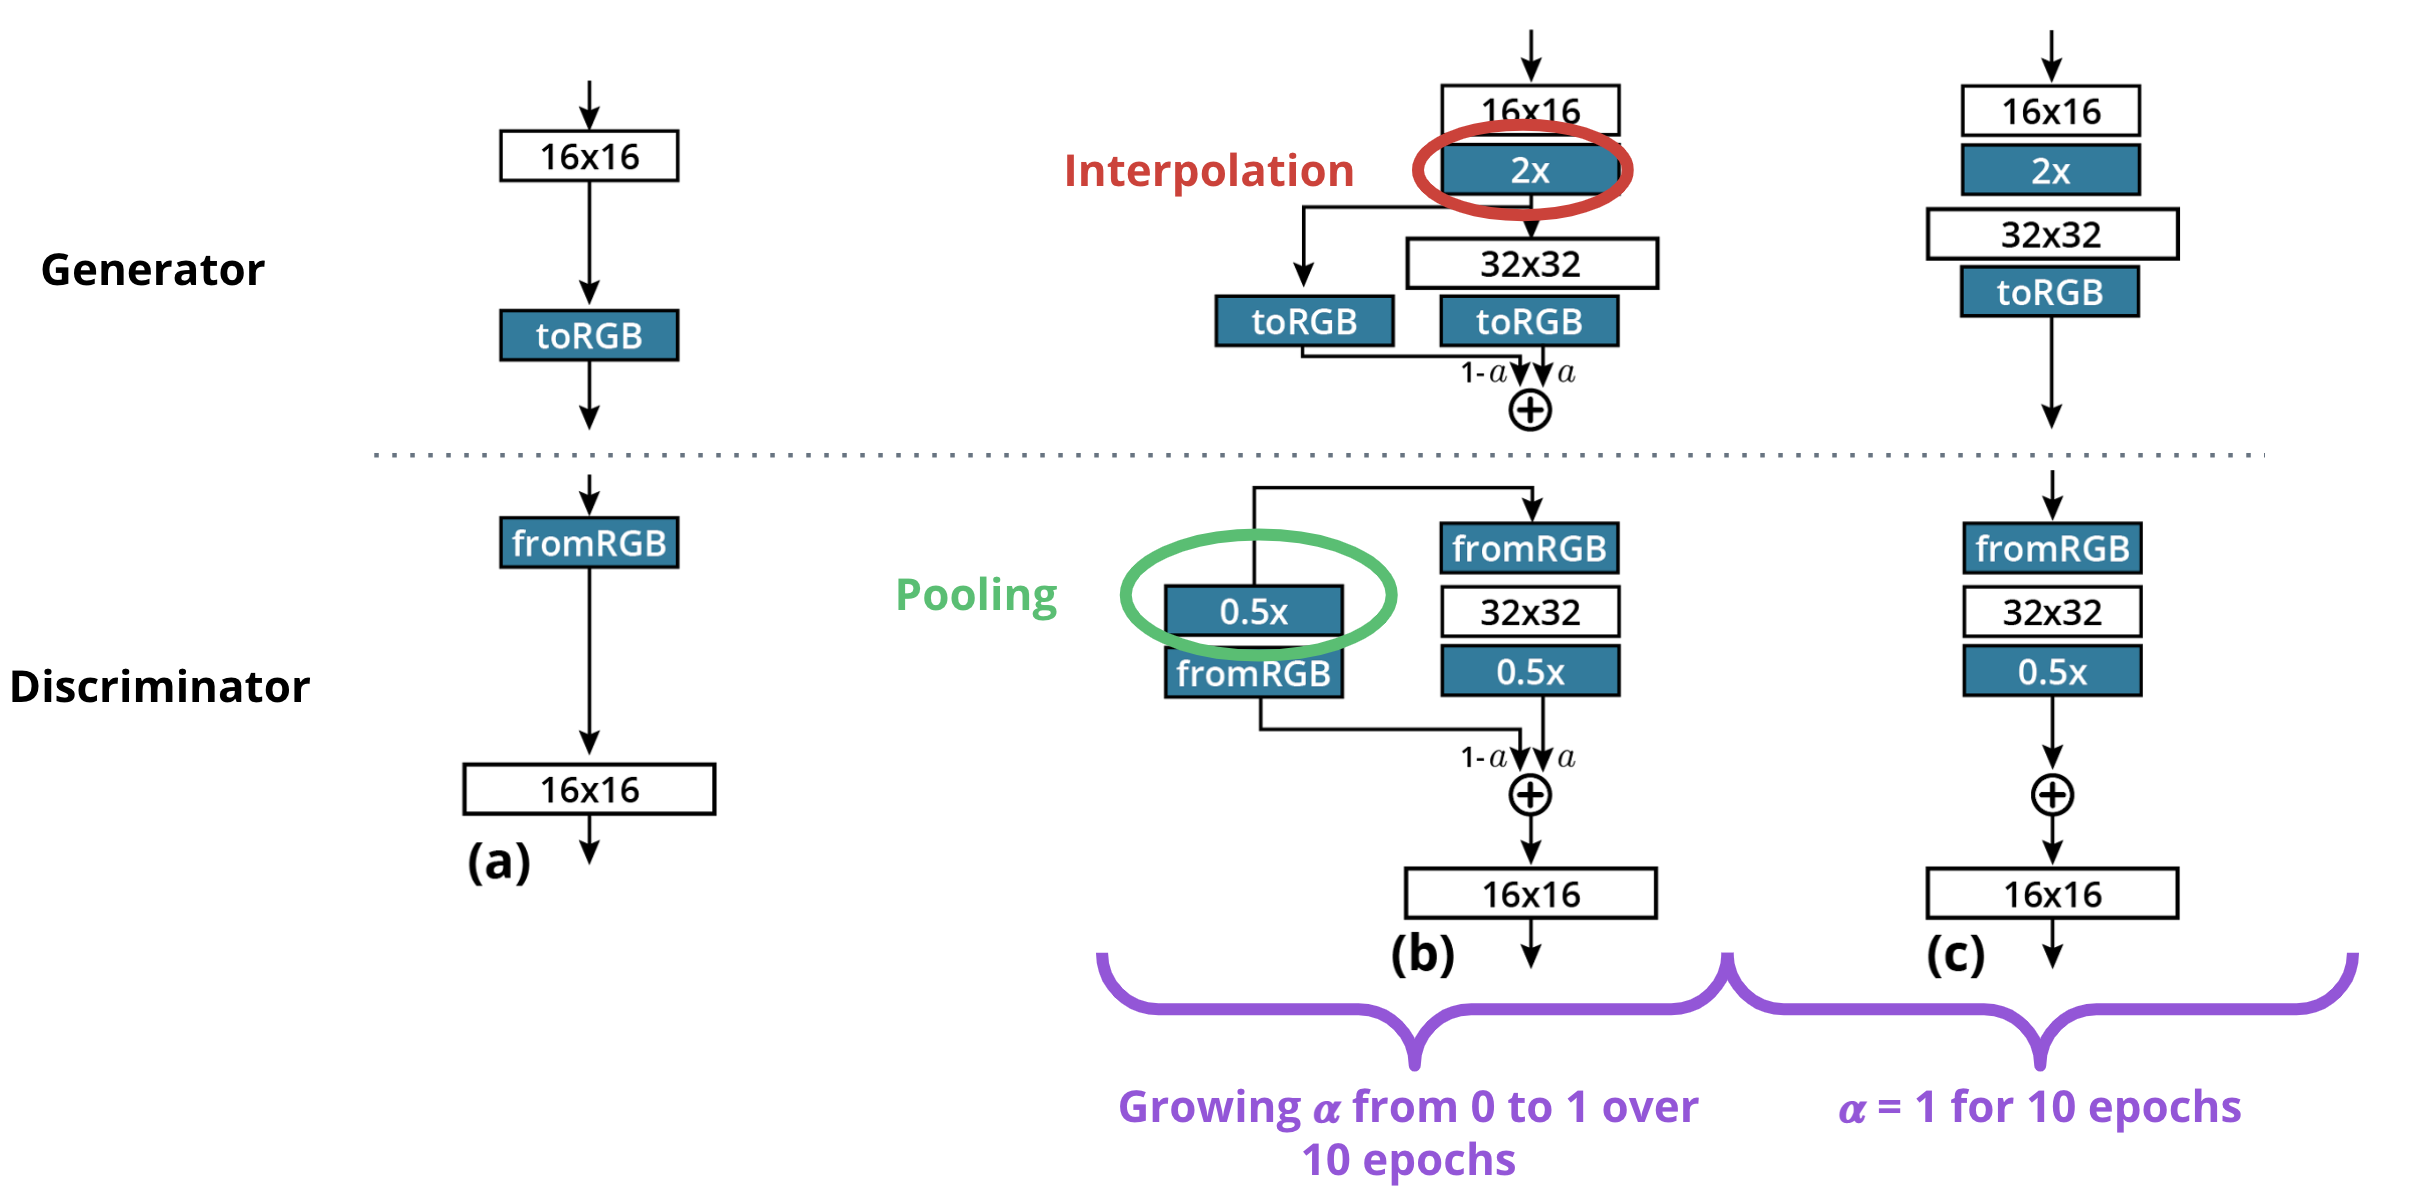
\includegraphics[width=1\linewidth]{img//genAdvNet//modernGAN/layer_fading2.png}

The \lstinline{toRGB} and
\lstinline{fromRGB} layers are the layers projecting the
feature vector to the RGB space (HxWx3) and the layer doing the
opposite, respectively. \newline

Let's look at the example: 
\begin{enumerate}[label=\textbf{(\alph*)}]
    \item the network is currrently training at 16x16 resolution, meaning that the generated images are 16x16x3
    \item we are adding two new layers to train at 32x32 resolution. However, we are fading the new layers by doing the following:
    \begin{itemize}
        \item for the generator, we take the output of the 16x16 layer and use nearest neighbor image resize to double its resolution to 32x32. The same output will also be fed to the 32x32 layer. Then we calculate the output of the network by doing a weighted sum of \((1- \alpha)\) the upsampled 16x16 image and \(\alpha\) the 32x32 layer output.
        \item for the discriminator, we do something similar but to reduce the resolution, we use an average pooling layer
        \item the network trains for N epochs at each resolution. During the first \(N/2\) epochs, we start with \(/alpha = 0\) and increase alpha linearly to \(/alpha = 1\). Then we train for the remaining \(N/2\) epochs with \(/alpha = 1\).
    \end{itemize}
    \item the network is now training at 32x32 resolution
\end{enumerate}

\subsubsection{Exercerise}
In this exercise, you will implement the Generator of the ProGan model. To make your life easier, I already implemented two torch modules: \lstinline{GeneratorFirstBlock} and \lstinline{GeneratorBlock}. 
\begin{itemize}
    \item The \lstinline{GeneratorFirstBlock} module takes the the latent vector as input and outputs a multi-dimensional feature maps
    \item the \lstinline{GeneratorBlock} module correspond to each layer added when increasing the resolution
\end{itemize}

\textbf{Notes:} In the paper, the authors are using a new type of normalization, called PixelNormalization. I encourage you to read the paper but for the sake of simplicity, I did not add any normalization here.

\begin{lstlisting}[language=Python]
import numpy as np
import torch
import torch.nn as nn
\end{lstlisting}

\begin{lstlisting}[language=Python]
class GeneratorFirstBlock(nn.Module):
    """
    This block follows the ProGan paper implementation.
    Takes the latent vector and creates feature maps.
    """
    def __init__(self, latent_dim: int):
        super(GeneratorFirstBlock, self).__init__()
        # initial block 
        self.conv0 = nn.ConvTranspose2d(latent_dim, 512, kernel_size=4)
        self.conv1 = nn.Conv2d(512, 512, kernel_size=3, padding=1)
        self.activation = nn.LeakyReLU(0.2)

    def forward(self, x: torch.Tensor):
        # x is a (batch_size, latent_dim) latent vector, we need to turn it into a feature map
        x = torch.unsqueeze(torch.unsqueeze(x, -1), -1)
        x = self.conv0(x)
        x = self.activation(x)
        
        x = self.conv1(x)
        x = self.activation(x)
        return x
\end{lstlisting}

\begin{lstlisting}[language=Python]
class GeneratorBlock(nn.Module):
    """
    This block follows the ProGan paper implementation.
    """
    def __init__(self, in_channels: int, out_channels: int):
        super(GeneratorBlock, self).__init__()

        self.conv1 = nn.Conv2d(in_channels, out_channels, 3, padding=1)
        self.conv2 = nn.Conv2d(out_channels, out_channels, 3, padding=1)
        self.activation = nn.LeakyReLU(0.2)

    def forward(self, x: torch.Tensor):
        x = interpolate(x, scale_factor=2)
        x = self.conv1(x)
        x = self.activation(x)

        x = self.conv2(x)
        x = self.activation(x)
        return x
\end{lstlisting}

Using the above two blocks, you can implement the Generator module. The end resolution that we want to reach is 512x512 and we will start at a 4x4 resolution.

\subsubsection{init}
The \lstinline{__init__} method should contain enough blocks to work at full resolution. We are only instantiating the generator once! So you will need to: 
\begin{itemize}
    \item create one GeneratorFirstBlock module
    \item create enough GeneratorBlocks modules such that the final resolution is 512x512
    \item create one \lstinline{toRGB} layer per resolution.
\end{itemize}

The number of filters in each layer is controlled by the \lstinline{num_filters} function below.

\subsubsection{forward}
The forward method does the following: 
\begin{itemize}
    \item takes the latent vector, the current resolution and \lstinline{alpha} as input.
    \item run the latent vector through the different blocks and perform \lstinline{alpha} fading
\end{itemize}

In the original paper, the number of filters of convolution layers increases with depth. The\lstinline{num_filters} function below will help you programmatically increase the number of filters based on the stage (or depth) of the generator. A depth of 1 correspond to 4x4 resolution, a depth of 2 to an 8x8 resolution etc.

\begin{itemize}
    \item you can the torch \lstinline{interpolate} function to double the resolution of an image
    \item you can use the \lstinline{np.log2} function to map the resolution of the input image to a ``depth'' (or stage) level. For example, \lstinline{np.log2(512) = 9} and \lstinline{np.log2(4)} = 2.
    \item when training at 4x4 resolution, you should not perform \(\alpha-\)fading.
\end{itemize}

\begin{lstlisting}[language=Python]
import tests

from torch.nn.functional import interpolate
\end{lstlisting}

\begin{lstlisting}[language=Python]
def num_filters(stage: int, 
                fmap_base: int = 8192,
                fmap_decay: float = 1.0,
                fmap_max: int = 512): 
    """
    A small helper function to computer the number of filters for conv layers based on the depth.
    From the original repo https://github.com/tkarras/progressive_growing_of_gans/blob/master/networks.py#L252
    """
    return min(int(fmap_base / (2.0 ** (stage * fmap_decay))), fmap_max)
\end{lstlisting}

\begin{lstlisting}[language=Python]
class Generator(nn.Module):
    """
    Generator: takes a latent vector as input and output an image.
    args:
    - max_resolution: max image resolution
    - latent_dim: dimension of the input latent vector
    """
    def __init__(self, max_resolution: int, latent_dim: int):
        super(Generator, self).__init__()

        # following the original implementation
        resolution_log2 = int(np.log2(max_resolution))

        # layers blocks
        self.blocks = [GeneratorFirstBlock(latent_dim)]
        for res in range(1, resolution_log2 - 1):
            self.blocks.append(GeneratorBlock(num_filters(res), num_filters(res+1)))
        self.blocks = nn.ModuleList(self.blocks)

        # to rgb blocks
        self.to_rgb = [nn.Conv2d(num_filters(res), 3, kernel_size=1) for res in range(1, resolution_log2)]
        self.to_rgb = nn.ModuleList(self.to_rgb)

    def forward(self, x: torch.Tensor, current_res: int, alpha: float = 1.0):
        resolution_log2 = int(np.log2(current_res))

        # to rgb operation
        if current_res == 4:
            x = self.blocks[0](x)
            images_out = self.to_rgb[0](x)
        else:
            # blocks
            for block in self.blocks[:resolution_log2-2]:
                x = block(x)

            previous_img = self.to_rgb[resolution_log2-3](x)
            previous_img_scaled = interpolate(previous_img, scale_factor=2)

            x = self.blocks[resolution_log2-2](x)
            new_img = self.to_rgb[resolution_log2-2](x)
            images_out = new_img * alpha + (1 - alpha) * previous_img_scaled
        return images_out
\end{lstlisting}

\begin{lstlisting}[language=Python]
generator = Generator(max_resolution=512, latent_dim=128)
\end{lstlisting}

\begin{lstlisting}[language=Python]
tests.check_progan_generator(generator)
\end{lstlisting}

\begin{lstlisting}[language=Python]
\end{lstlisting}
